\chapter{Introducción}
\label{cap:intro}

La rotonda de Padre Anchieta (cuyo nombre oficial es «glorieta del Brasil») toma su nombre por la escultura en representación del beato José de Anchieta, colocada en el centro de la rotonda, y regalada por el pueblo brasileño en 1960~\cite{gallo_glorieta_2013}.

\begin{figure}[H]
    \centering
    \includegraphics[width=\textwidth]{report/images/padre-anchieta.png}
    \caption[Mapeado en 3D de la Rotonda del Padre Anchieta.]{Mapeado en 3D de la Rotonda del Padre Anchieta. Cortesía de Google Earth\protect\footnotemark}
    \label{fig:padre_anchieta_3d}
\end{figure}

\footnotetext{Véase \url{https://earth.google.com/web/@28.48023943,-16.31770104,534.93762391a,251.9187181d,35y,-46.25428648h,74.81244137t,0r}}

La popularidad de la rotonda se explica por su posición estratégica, rodeada de viviendas, comercios, dos campus universitarios de la Universidad de La Laguna (Central y Anchieta), y por la cual pasa una de las principales autopistas de la isla, la TF-5; además de conectar otras cuatro vías: la Carretera de la Esperanza (TF-24), la Carretera de Geneto (TF-263), la Avenida de la Trinidad y la Avenida Astrofísico Francisco Sánchez. Sin embargo, los orígenes de la rotonda son considerablemente más humildes (véase la Figura~\ref{fig:anchieta_ev}).

Hoy en día, y después de varias obras, la rotonda ha incrementado considerablemente su tamaño y el tráfico que circula a través de ella, especialmente en horas punta. Es normal que en dichas horas se produzcan retenciones muy importantes y, en determinadas situaciones, un bloqueo total del tráfico; a veces durante horas (véase~\cite{gulesserian_vuelven_2018}, a modo de ejemplo). Las grandes cantidades de tráfico que absorbe la rotonda, y los bloqueos y ralentizaciones que se producen como consecuencia, tienden a afectar al tráfico de la TF-5, causando retenciones a la altura de la rotonda.

La optimización del tráfico en la rotonda se convierte, por tanto, en un asunto de primer orden respecto de la movilidad en la isla. La rotonda da una vía a los estudiantes tanto del norte como del sur que van a clase, a los trabajadores que se dirigen hacia La Laguna y hacia Santa Cruz; y en general a una gran cantidad de trayectos entre ambas ciudades y el norte de la isla que no puede dejarse desatendida.

\begin{figure}[h]
    \centering
    \begin{subfigure}[t]{.49\textwidth}
      \centering
      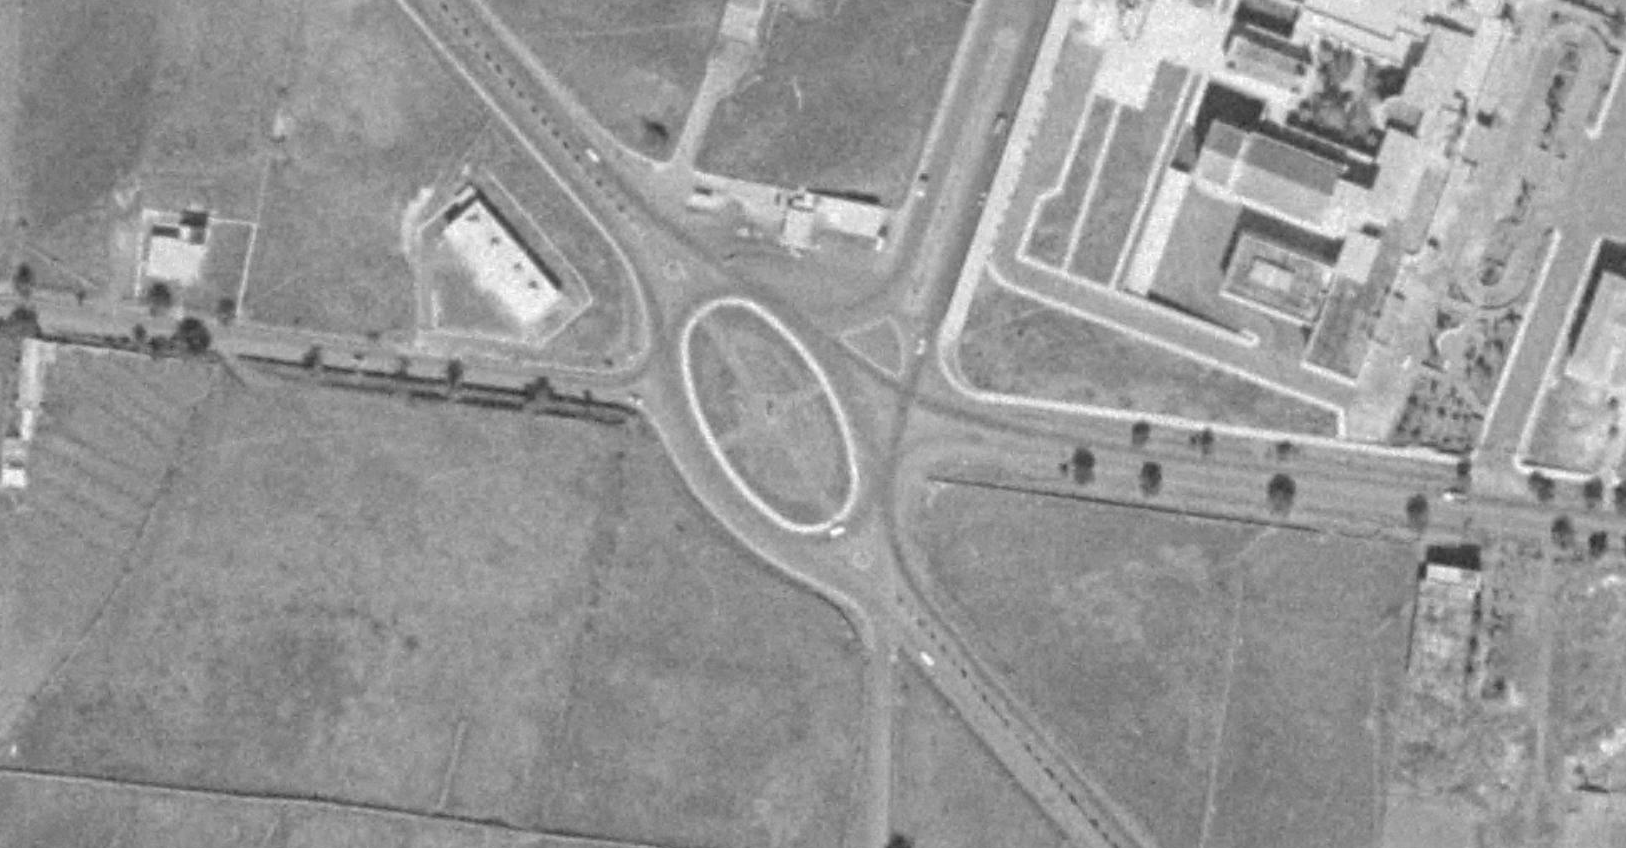
\includegraphics[width=\textwidth]{report/images/amp-anchieta-1964.png}
      \caption{1964}
      \label{fig:anchieta1964}
    \end{subfigure}
    \hfill
    \begin{subfigure}[t]{.49\textwidth}
      \centering
      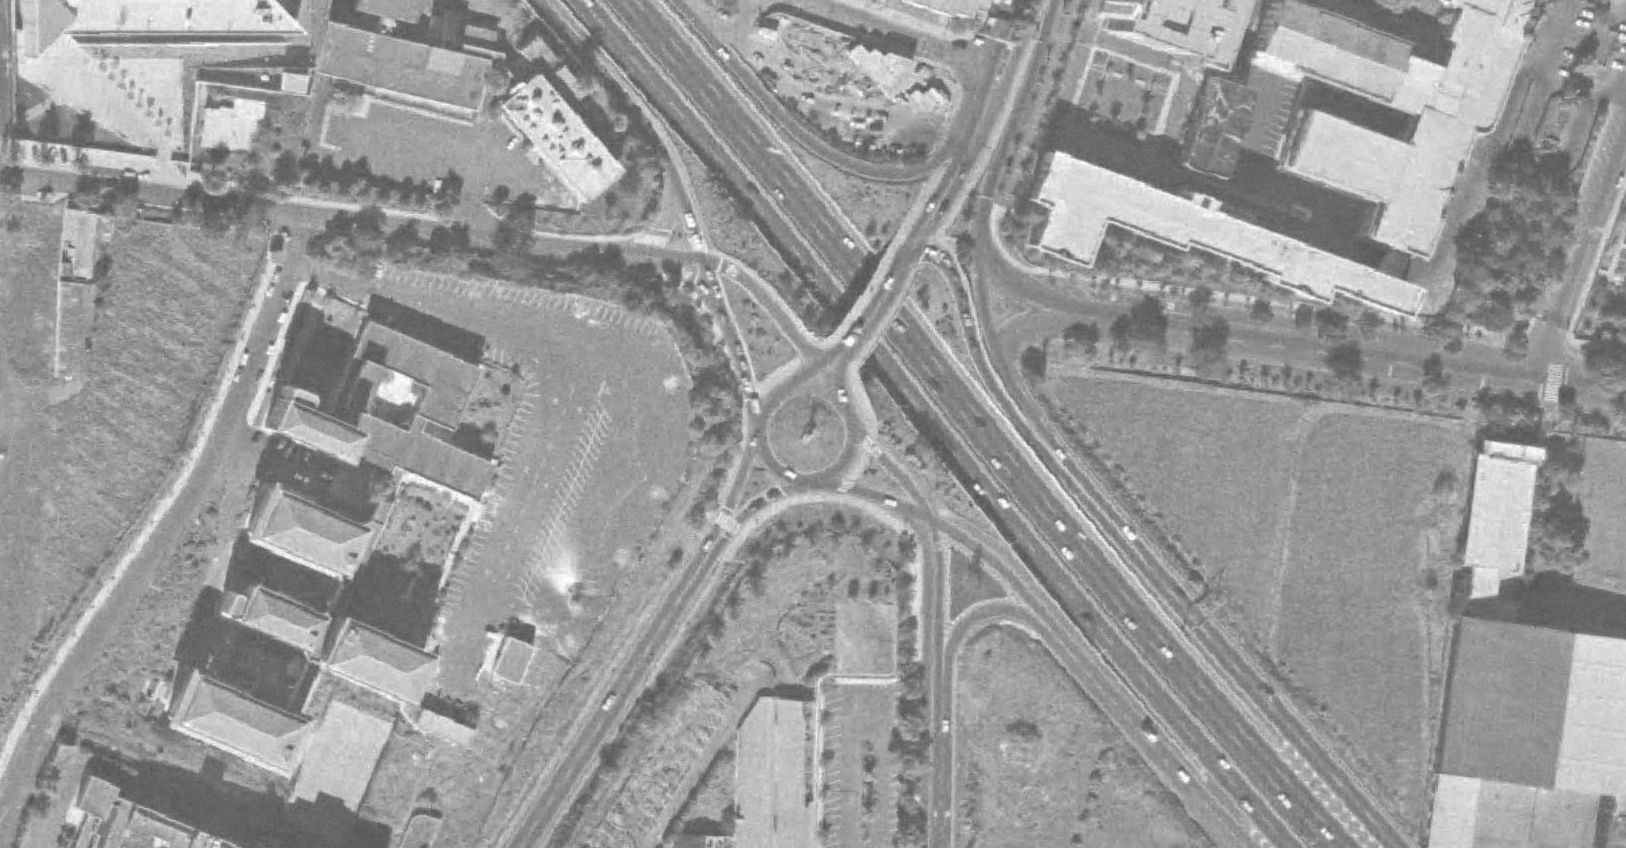
\includegraphics[width=\textwidth]{report/images/amp-anchieta-1994.png}
      \caption{1994}
      \label{fig:anchieta1994}
    \end{subfigure}
    \vspace{0.7cm}
    \begin{subfigure}[t]{.49\textwidth}
      \centering
      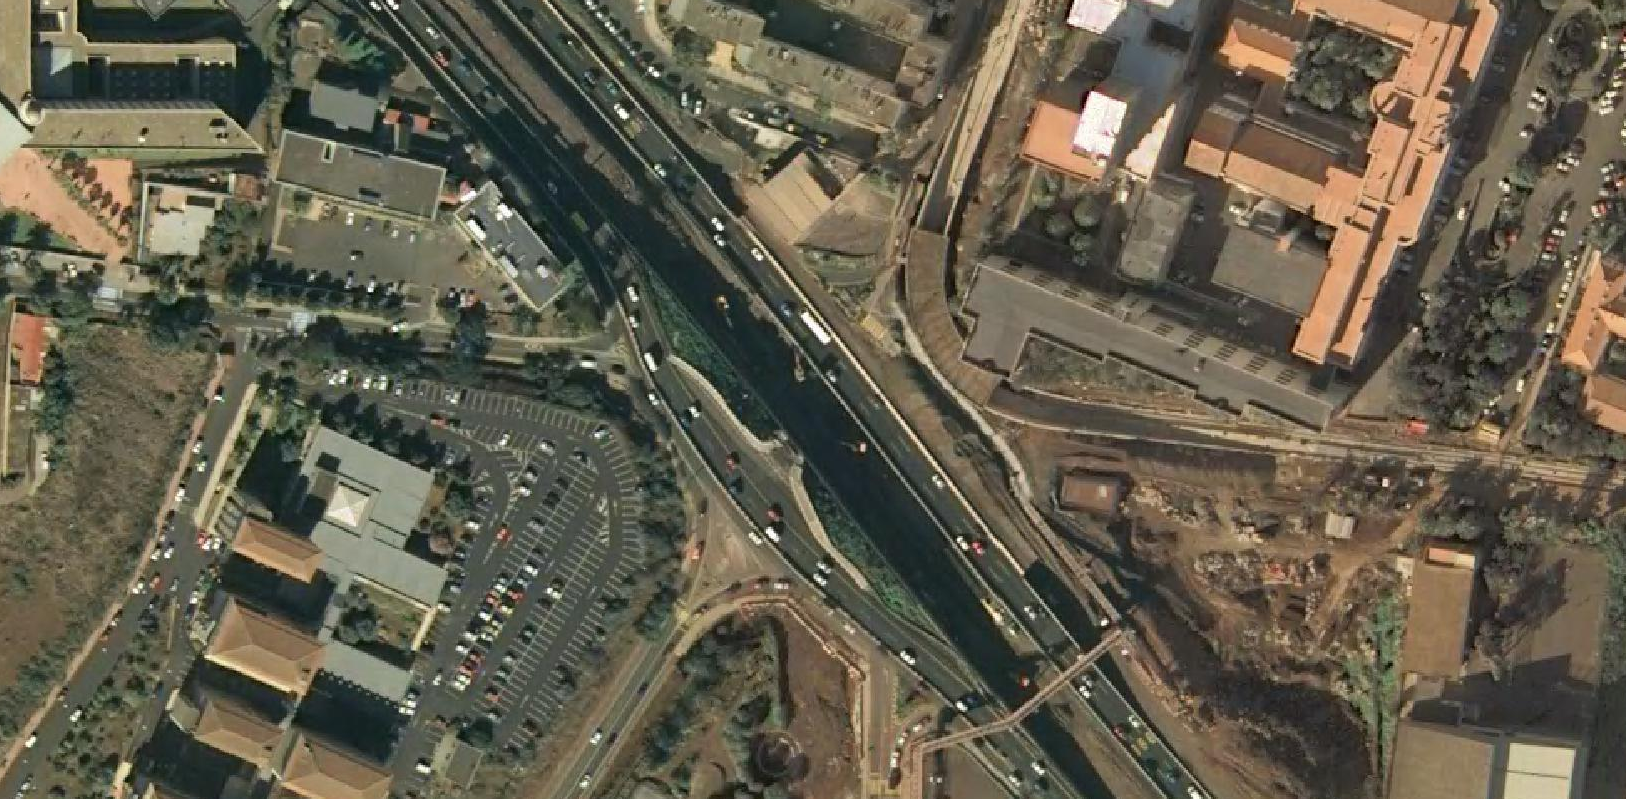
\includegraphics[width=\textwidth]{report/images/amp-anchieta-2006.png}
      \caption{2006 (en obras)}
      \label{fig:anchieta2006}
    \end{subfigure}
    \hfill
    \begin{subfigure}[t]{.49\textwidth}
      \centering
      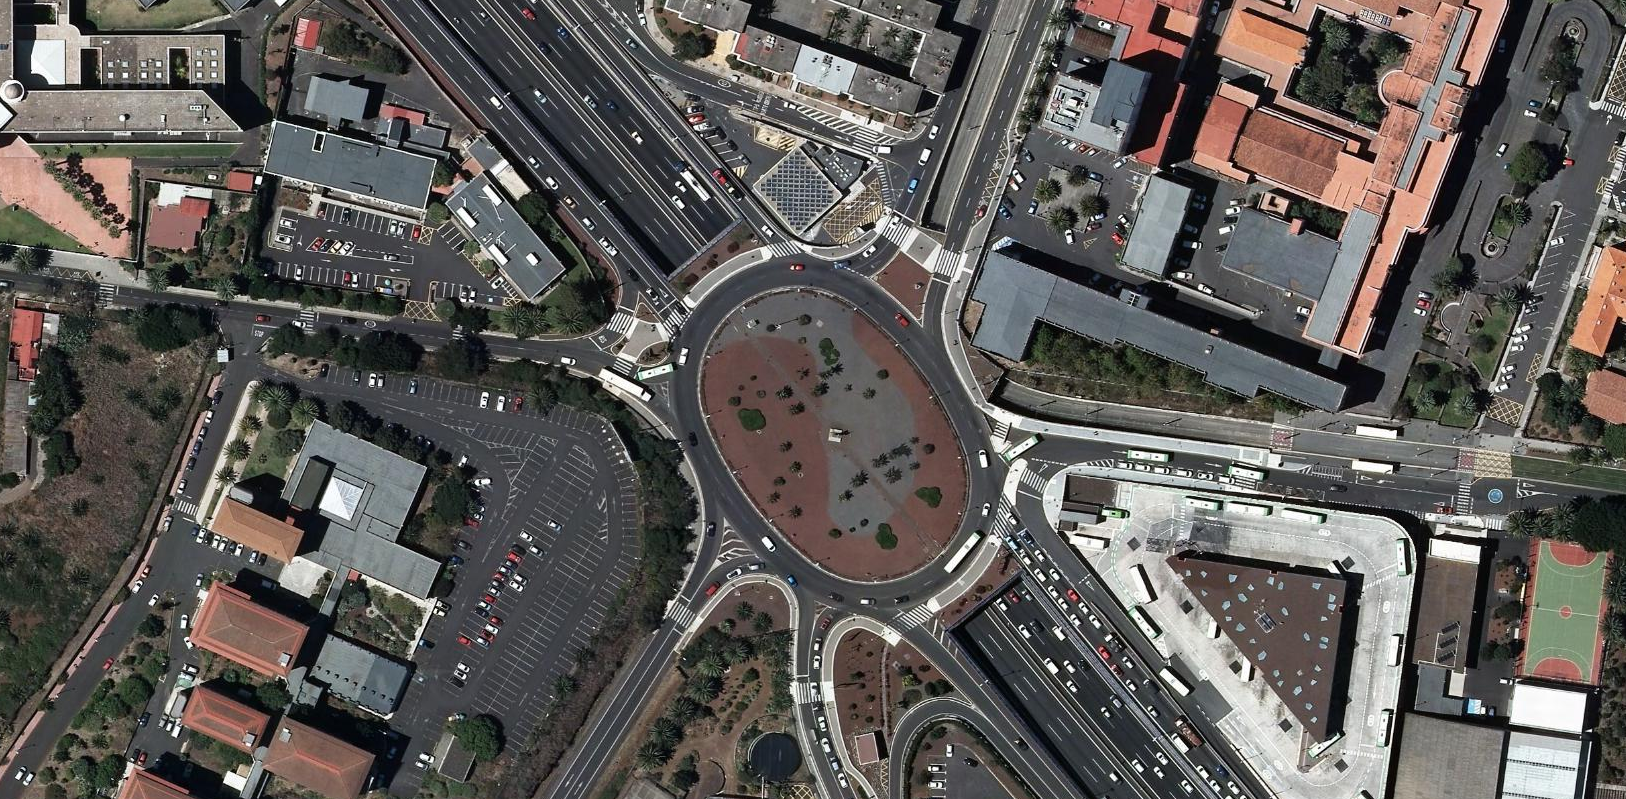
\includegraphics[width=\textwidth]{report/images/amp-anchieta-2019.png}
      \caption{2019}
      \label{fig:anchieta2019}
    \end{subfigure}
    \caption[Evolución de la rotonda de Padre Anchieta a lo largo de los años.]{Evolución de la rotonda de Padre Anchieta a lo largo de los años. Fotografías cortesía de GRAFCAN\protect\footnotemark}
    \label{fig:anchieta_ev}
\end{figure}

\footnotetext{Véase \url{https://visor.grafcan.es/visorweb/}}

Las autoridades de la isla no son ajenas al problema de tráfico que plantea la rotonda. El Cabildo de Tenerife, organismo de cuya competencia depende la rotonda, y el Gobierno de Canarias, de cuya competencia depende la TF-5, han planteado varias medidas, de entre las cuales cabe mencionar:

\begin{itemize}
    \item El soterramiento de la TF-24 en dirección hacia Santa Cruz (a la espera de ejecutar el proyecto)~\cite{dia_cabildo_2019}.
    \item La construcción de una pasarela de peatones sobre la rotonda~\cite{rozas_pasarela_2019}.
    \item La potenciación del vehículo compartido y el transporte público: creación de carriles BUS-VAO en la TF-5~\cite{20minutos_gobierno_2019}.
    \item Las propuestas para la construcción de nuevas líneas de tranvía~\cite{redaccion_de_eldiarioes_cabildo_2020}.
\end{itemize}

Sin embargo, todas las medidas mencionadas suponen un cargo importante al erario público, suponen una carga administrativa importante (por todos los procesos de licitación y control que han de realizarse), llevan mucho tiempo construirlas y mientras dure el proceso resultarán un incordio para los conductores y usuarios de la vía.


\section{Objetivos}

Con la elaboración de este proyecto lo que se propone es la instalación de semáforos en la rotonda, cuyas duraciones de fase se optimicen mediante un algoritmo evolutivo. De esta forma, se podrá comprobar si con la instalación de estos semáforos es posible mejorar la circulación del tráfico en función de determinados parámetros como: la duración media de los trayectos de los vehículos, la velocidad media de los vehículos, la cantidad de vehículos que han logrado completar su trayecto en
un tiempo determinado, etc.
% Gara
%una hora, etc.

El problema que se pretende abordar no es otro que el de la planificación de la duración de las fases de los semáforos, más conocido como el \textit{Traffic Light Scheduling Problem} (TLSP). Este problema de optimización plantea cuánto deberían durar las fases de los semáforos de uno o varios cruces para mejorar la circulación con respecto a varios parámetros; el más habitual de ellos siendo el tiempo medio de viaje de un grupo de vehículos desde un origen hasta el destino. Otros parámetros, como la distancia media o la contaminación de los vehículos también pueden ser tenidos en cuenta a la hora de evaluar el comportamiento de las distintas configuraciones semafóricas.

En comparación con las medidas antes mencionadas, la que se propone en este trabajo supone un coste considerablemente más bajo, no molestaría tanto a los conductores durante la instalación (la cual sería también mucho más corta y sencilla) y plantea una solución muy interesante que podría ser reaprovechada para otras vías sin coste alguno (si ya tuvieran semáforos instalados).

Para llevar a cabo el proyecto, se han empleado principalmente las dos herramientas siguientes:

\begin{itemize}
    \item La primera de ellas es \textit{SUMO}~\cite{lopez_microscopic_2018}, un simulador de tráfico microscópico que nos permitirá evaluar cómo se comporta el tráfico en la rotonda de Padre Anchieta, con datos de tráfico provistos por el Cabildo de Tenerife.
    \item La segunda es \textit{Genetics.js}~\cite{abrante_dorta_framework_2019}, una librería orientada a algoritmos evolutivos (en particular, algoritmos genéticos) programada en \textit{TypeScript}.
\end{itemize}


\section{Optimización mediante algoritmos evolutivos}

Los algoritmos evolutivos toman como guía la evolución biológica y la llevan al campo de la optimización. A diferencia de otros métodos, esta clase de algoritmos busca ofrecer mejores resultados mediante la evolución de los individuos de una población, haciéndolos mutar, combinando características entre ellos y seleccionando los mejores candidatos a optar a solución de un problema~\cite{eiben_introduction_2003} (normalmente, de optimización no lineal con un amplio espacio de búsqueda), donde otros algoritmos tardarían demasiado o serían directamente inviables.

Este tipo de algoritmos se componen de varios elementos~\cite{eiben_introduction_2003}:

\begin{itemize}
    \item \textbf{Representación.} Es la manera en que representamos los individuos. Para el caso que aquí nos atañe, un individuo es una intersección vial con un conjunto de semáforos. La duración de cada una de las fases de esos semáforos, así como los retardos, se representan como un vector de números. Cada individuo es una posible solución.
    \item \textbf{Función de evaluación (fitness).} Devuelve un valor, a partir de un individuo, que determina qué tan bueno es como solución al problema.
    \item \textbf{Población}. Conjunto de individuos. Es útil para determinar cuantos individuos vamos a forzar a competir entre sí en una generación.
    \item \textbf{Mecanismo de selección de padres.} Se corresponde con los criterios tenidos en cuenta a la hora de determinar cuáles queremos que sean los individuos que se reproducirán en la generación, normalmente de carácter estocástico.
    \item \textbf{Operadores (recombinación y mutación).} Determinan la manera en que se alteran los individuos de la población.
    \item \textbf{Mecanismo de selección de supervivientes (reemplazo).} Se centra en seleccionar a los individuos que formarán parte de la siguiente generación de entre la población padre y la población hija a partir de los operadores genéticos. Este mecanismo, a diferencia del de selección de padres, suele ser un método determinista basado en el fitness.
    \item \textbf{Inicialización y terminación.} Finalmente, debemos determinar de qué manera queremos iniciar el algoritmo (normalmente, con individuos generados aleatoriamente) y cómo queremos terminarlo (por ejemplo, tras un número determinado de iteraciones, o en función de un umbral, tomando como guía el \textit{fitness} o la diversidad entre individuos).
\end{itemize}


% Gara:
% Yo creo que empezaría la frase diciendo algo como "este tipo de algoritmos se utilizarán para optimizar los tiempos y fases del conjunto de semáforos
Este tipo de parámetros se pueden emplear en la función de evaluación del algoritmo evolutivo para calcular el valor que correspondería a un individuo; en este caso, un conjunto de semáforos. En el capítulo~\ref{cap:simulacion} se detallarán los parámetros tenidos en cuenta en dicha función, así como otros aspectos relevantes relacionados con el planteamiento del problema.

Así pues, el TLSP busca solventar los tiempos que han de asignarse a cada fase de un conjunto de semáforos, buscando que tales tiempos se ajusten a determinadas restricciones y que sean óptimos. Una fase de un conjunto de semáforos es un momento determinado en que cada semáforo alumbra un color distinto. Por ejemplo: tomando en cuenta dos semáforos $S_1$ y $S_2$, una fase en concreto se correspondería con el semáforo $S_1$ en rojo y el semáforo $S_2$ en ámbar.

Cuando tratamos con varios conjuntos de semáforos es normal que algunas ciudades planteen una sincronización entre estos a través de retardos, denominadas <<oleadas de verde>>, lo que en determinadas circunstancias optimiza la circulación de vehículos. Este retardo también se ha tenido en cuenta en la evaluación del algoritmo.

Para obtener estos valores es necesario simular el comportamiento de los vehículos con las distintas configuraciones de semáforos. Para esto se ha empleado SUMO, un simulador de tráfico microscópico de código abierto, que nos proveerá con los argumentos necesarios para la función de evaluación.

La obtención de los datos necesarios para realizar las simulaciones, como el mapa de la localización que queremos simular, así como los datos de circulación de los vehículos, han sido obtenidos: de un lado, de \textit{OpenStreetMap} (para el caso del mapa); y de otro, del Cabildo de Tenerife (para el caso de los datos de circulación de la zona en cuestión). De esto se hablará con extensión en los siguientes capítulos, pues el tratamiento de estos datos conforma una parte importante del proyecto. La Figura~\ref{fig:evolutionary_alg_graph} sintetiza el proceso de trabajo principal del proyecto descrito en estos párrafos.
% Gara: creo que primero pondría la gráfica y luego empezaría a explicar a partir de ella, indicando el capítulo/s en el que se desarrolla cada paso...

\begin{figure}[!t]
    \centering
    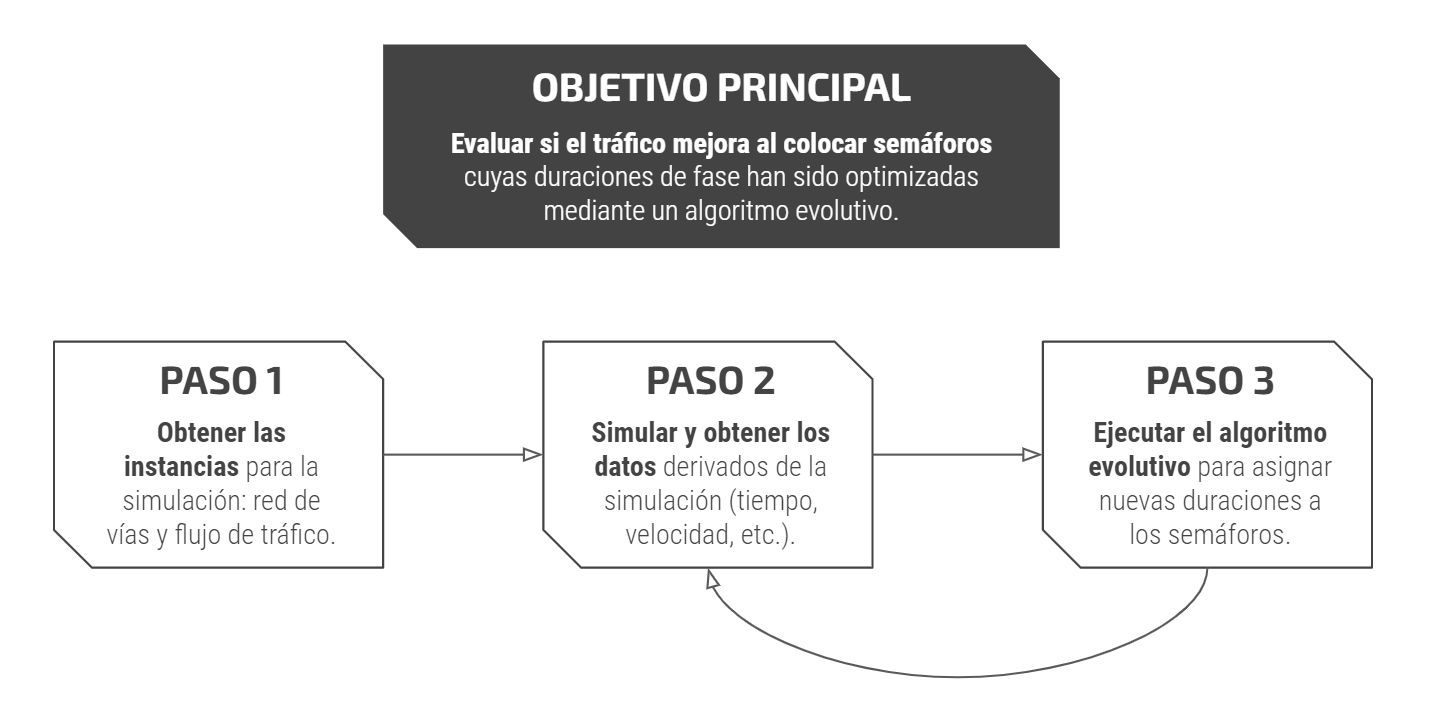
\includegraphics[width=\textwidth]{report/images/evolutionary_alg_graph.png}
    \caption{Gráfica del proceso general del trabajo.}
    \label{fig:evolutionary_alg_graph}
\end{figure}

La zona seleccionada para llevar a cabo la simulación ha sido la de la glorieta del Brasil (más conocida como la rotonda del Padre Anchieta), sita en San Cristóbal de La Laguna. La elección de esta zona en particular viene determinada por la gran cantidad de tráfico que absorbe cada día, al estar situada en el corazón del municipio, al haber una gran variedad de viviendas, comercios y lugares de trabajo en las zonas conexas, así como por la presencia de dos campus universitarios pertenecientes a la Universidad de La Laguna. La rotonda no tiene semáforos, por lo cual en este proyecto se han planteado varias configuraciones semafóricas.

Por tanto, lo que se plantea en este proyecto es la obtención de una instancia real, con datos de tráfico incluidos, de la rotonda del Padre Anchieta. Los resultados de la simulación del tráfico realizada por SUMO en dicha instancia servirán de entrada a un algoritmo evolutivo para evaluar si, incluyendo semáforos en la rotonda y optimizando la duración de las fases, es posible mejorar la circulación en función de los parámetros especificados.


\section{Trabajos previos relacionados}

El planteamiento aquí propuesto ya ha sido tratado desde distintas perspectivas por otros autores en los que se basa este trabajo, de entre los que cabe resaltar los siguientes:

\begin{itemize}
    \item Segredo \textit{et al.}~\cite{segredo_optimising_2019}. El artículo versa sobre el TLSP y el empleo de varios optimizadores mono y multi-objetivos basados en la diversidad, por ser mucho más eficientes y, en consecuencia, ser capaces de lidiar con zonas significativamente más grandes de ciudades como Berlín, París, Estocolmo o Málaga, llegando a simular casi 1000 intersecciones y más de 2600 vehículos.
    \item Sánchez \textit{et al.}~\cite{sanchez_applying_2008}. El artículo, de 2008, versa también sobre el TLSP pero aplicado a las Ramblas, en Santa Cruz de Tenerife. El autor, con la optimización propuesta de las duraciones de las fases de los semáforos, consigue mejoras notables en la circulación del tráfico.
    \item Dorta Acosta~\cite{dorta_acosta_simulacion_2019}. En este caso se trata de un TFG de un compañero de la Escuela Superior de Ingeniería y Tecnología, que versa sobre la instalación de semáforos inteligentes en la rotonda de Padre Anchieta.
\end{itemize}

